\newpage
\section{Praktischer Teil: Kalkulation eines neuen E-Bike-Modells in SAP-CO} \label{infos}
\subsection{Fallbeispiel}
Szenario: Global Bike möchte sein Produktportfolio um ein neues E-Bike-Modell erweitern. Für die Entscheidung über die Einführung und Preisgestaltung soll eine Kalkulation der voraussichtlichen Produktkosten erstellt werden.
 Um dieses Vorhaben in die Tat umzusetzen, müssen folgende Schritte befolgt werden:
\\
\begin{figure}[H]
    \caption{Prozessverlauf Fallstudie}\label{fig:process}
    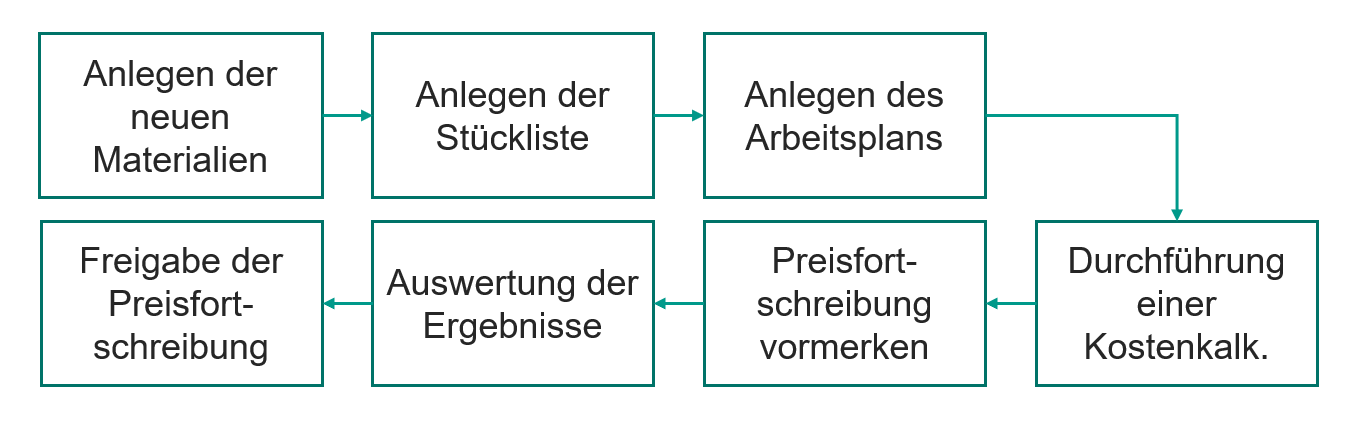
\includegraphics[width=0.9\textwidth]{ablauf}
    \\
    Quelle: Eigene Darstellung
\end{figure}
    
\begin{enumerate}
    \item \textbf{Anlegen der neuen Materialien}\\
    Das geplante E-Bike-Modell besteht aus verschiedenen Materialien. Die meisten dieser hat Global Bike bereits im System angelegt, da sie auch im Deluxe Touring Bike verbaut sind. Für das neue Modell müssen jedoch noch ein Elektromotor, ein Akku, und ein Ladekabel angelegt werden.
    \item \textbf{Anlegen der Stückliste}\\
    Die Stückliste enthält alle Materialien, die für die Produktion des E-Bikes benötigt werden. Sie gibt außerdem Auskunft darüber in welcher Menge die Materialien benötigt werden.
    \item \textbf{Anlegen des Arbeitsplans}\\
    Der Arbeitsplan enthält alle Arbeitsschritte, die für die Produktion des E-Bikes notwendig sind. Er gibt außerdem Auskunft darüber, wie lange die einzelnen Arbeitsschritte dauern und welche Ressourcen benötigt werden.
    \item \textbf{Durchführung der Kostenkalkulation}\\
    Die Kostenkalkulation gibt Auskunft darüber, wie hoch die voraussichtlichen Produktionskosten für das E-Bike sind. Sie setzt sich aus den Materialkosten, den Fertigungskosten und den Gemeinkosten zusammen. Dinge wie Vermarktungskosten oder Gewinnmarge sind hier noch nicht enthalten.
    \item \textbf{Vormerken der Preisfortschreibung}\\
    Der kalkulierte Preis wird zunächst als Vorschlag für die Preisfortschreibung vorgemerkt und in den Materialstammsatz übertragen. Dies ist der erste von zwei Schritten, aus welchen die Preisfortschreibung besteht.
    \item \textbf{Auswertung der Ergebnisse}\\
    Die Ergebnisse der Kostenkalkulation werden analysiert. Dabei wird geprüft, ob die kalkulierten Kosten in etwa den erwarteten Kosten entsprechen und ob auf dieser Basis ein auf dem Markt konkurrenzfähiger Preis festgelegt werden kann.
    \item \textbf{Freigabe der Preisfortschreibung}\\
    Nachdem die Ergebnisse der Kostenkalkulation analysiert wurden, und die Entscheidung positiv ausgefallen ist, wird die Preisfortschreibung freigegeben. Dies ist der zweite Schritt, aus welchen die Preisfortschreibung besteht und der Preis wird hier endgültig festgelegt.
\end{enumerate}
    
\subsection{Dokumentation und Erklärung}
Im Folgenden werden die einzelnen Schritte des Prozesses anhand ausgewählter Grafiken genauer erläutert und dokumentiert. Für die Durchführung der Schritte wurde SAP-Fiori verwendet. Außerdem wurde diese Fallstudie
 mit der Kennung 201 durchgeführt. Wenn man die Fallstudie nachmachen möchte, muss man die Stellen an welchen 201 angehängt ist durch die eigene Kennung ersetzen.
\subsubsection{Anlegen der neuen Materialien}
Da noch nicht alle benötigten Bauteile für das neue E-Bike-Modell, sowie das E-Bike selbst im System vorhanden sind, müssen diese zunächst angelegt werden.
 Hierfür muss man unter dem Reiter \textit{Controlling} zur Karte \textit{Material anlegen} navigieren und diesen auswählen. Nun öffnet sich das Fenster 
 \textit{Material anlegen (Einstieg)}. Hier müssen man nun bei \textit{Material} das Material eingeben, welches angelegt werden soll. Im Beispiel wird hier mit dem Elektromotor für das E-Bike gestartet. Daher muss
 das Material \textit{EBEN1201} abgegeben werden. Weiterhin muss noch die passende
 \textit{Branche}, im Beispiel \textit{Maschinenbau}, und eine passende \textit{Materialart}, im Beispiel \textit{Rohstoff}, ausgewählt werden. Sollte schon ein Material im System vorhanden sein, 
 welches sich als Vorlage für das neue Material eignet, kann dies im Bereich \textit{Kopieren aus...} bei \textit{Material} angegeben werden. In diesem Fall werden Felder aus der Vorlage übernommen.
\begin{figure}[H]
    \caption{Anlegen des Materials}\label{fig:material}
    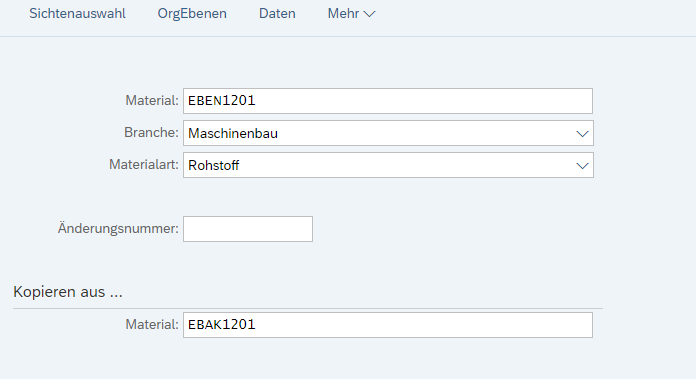
\includegraphics[width=0.9\textwidth]{Material Anlegen}
    \\
    Quelle: Eigene Darstellung
\end{figure}
Wenn alles richtig angegeben wurde, kann man nun auf \textit{Weiter} klicken und muss in dem neu geöffneten Fenster mit Titel \textit{Sichtenauswahl} die Sichten
 \textit{Grunddaten 1}, \textit{Grunddaten 2}, \textit{Disposition 1} und \textit{Buchhaltung 1} selektieren.
\begin{figure}[H]
    \caption{Sichtenauswahl}\label{fig:sichtenauswahl}
    \includegraphics[width=0.9\textwidth]{Sichtenauswahl}
    \\
    Quelle: Eigene Darstellung
\end{figure}
Im nächsten Fenster muss jetzt noch das Werk angeben. Für das Beispiel wird das Werk in Dallas namens \textit{DL00} gewählt. 
\begin{figure}[H]
    \caption{Werk auswählen}\label{fig:werk}
    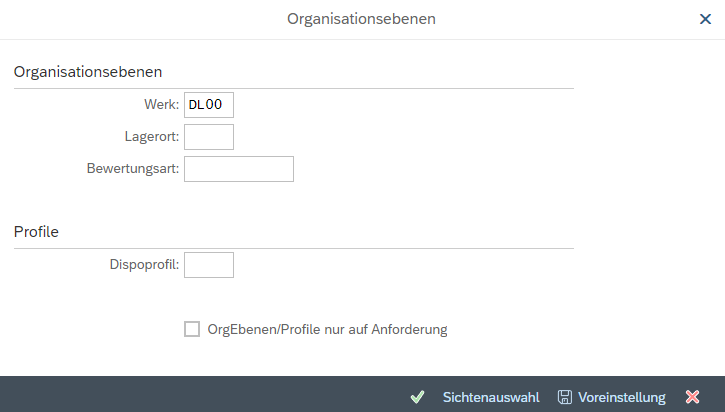
\includegraphics[width=0.9\textwidth]{Werk}
    \\
    Quelle: Eigene Darstellung
\end{figure}
Im folgenden Fenster können jetzt die passenden Daten für das Material eingegeben werden. In der Sicht \textit{Grunddaten 1} kann man allgemeine Daten zum
 Material angeben. In der Fallstudie wird \textit{E-Bike Motor} als \textit{Bezeichnung} und \textit{EA} als \textit{Basismengeneinheit} verwendet, was so viel wie Stück bedeutet.
\begin{figure}[H]
    \caption{Grunddaten 1 - Bezeichnung und allgemeine Daten}\label{fig:grunddaten1.1}
    \includegraphics[width=0.9\textwidth]{Grunddaten1.1}
    \\
    Quelle: Eigene Darstellung
\end{figure}
 
 Weiterhin können Abmessungen angegeben werden. Im Beispiel wird hier \textit{1000} für \textit{Bruttogewicht} und \textit{Nettogewicht} sowie \textit{G} für die \textit{Gewichtseinheit} eingegeben.

\begin{figure}[H]
    \caption{Grunddaten 1 - Abmessungen}\label{fig:grunddaten1.2}
    \includegraphics[width=0.9\textwidth]{Grunddaten1.2}
    \\
    Quelle: Eigene Darstellung
\end{figure}

Weiter geht es im Bereich \textit{Disposition 1}. Hier wird im Beispiel als \textit{Dispositionsmerkmal} \textit{ND} angegeben. ND steht für \textit{keine Disposition} und wird hier der Einfachheit halber verwendet. 
Das passende Dispositionsmerkmal unterscheidet sich je nach Szenario.

\begin{figure}[H]
    \caption{Disposition 1}\label{fig:disposition1}
    \includegraphics[width=0.9\textwidth]{Disposition1}
    \\
    Quelle: Eigene Darstellung
\end{figure}

Weiterhin wird unter \textit{Disposition 3} bei Verfügbarkeitsüberprüfung \textit{02} ausgewählt.

\begin{figure}[H]
    \caption{Disposition 3}\label{fig:disposition3}
    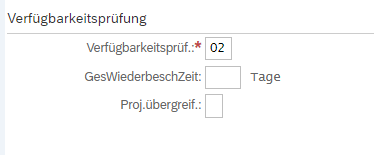
\includegraphics[width=0.9\textwidth]{Disposition3}
    \\
    Quelle: Eigene Darstellung
\end{figure}

Zudem müssen im Reiter \textit{Buchhaltung 1} noch \textit{Bewertungsklasse} und die passenden Kosten für das Material angeben. Hierfür werden in der Fallstudie unter dem Reiter \textit{Bewertungsklasse} die Klasse \textit{3000} (Rohstoffe 1) und im Bereich \textit{Preise und Werte} die Felder \textit{Standardpreis} \textit{Per. VPreis} mit \textit{200} befüllt.

\begin{figure}[H]
    \caption{Buchhaltung 1}\label{fig:buchhaltung1}
    \includegraphics[width=0.9\textwidth]{Buchhaltung1}
    \\
    Quelle: Eigene Darstellung
\end{figure}

Dieser Vorgang muss für alle Materialien, die noch nicht im System vorhanden sind, wiederholt werden. Für das Beispiel sind dies der Akku, das Ladekabel und das E-Bike selbst.

\subsubsection{Anlegen der Stückliste}
Nachdem alle neuen Materialien im System angelegt wurden, muss nun die Stückliste für das E-Bike angelegt werden. Hierfür auf der Startseite unter dem
 Reiter \textit{Controlling} die Kachel \textit{Stückliste anlegen} gewählt werden. Im neuen Fenster muss man nun angeben, für welches Material man eine neue Stückliste anlegen will. In der Fallstudie wird im Feld \textit{Material} das neue E-Bike \textit{DXEB1201} angegeben. Weiterhin werden \textit{Werk} und \textit{Verwendung} mit \textit{DL00} für das Werk in Dallas und \textit{6} (Kalkulation) befüllt.
 Da alle Bauteile des Deluxe Tracking Bikes auch in dem neuen E-Bike verbaut sind, kann man hier die Stückliste des Deluxe Tracking Bikes als Vorlage verwenden.
 Hierfür muss man \textit{Vorlage kopieren...} wählen.

\begin{figure}[H]
    \caption{Stückliste anlegen}\label{fig:stueckliste}
    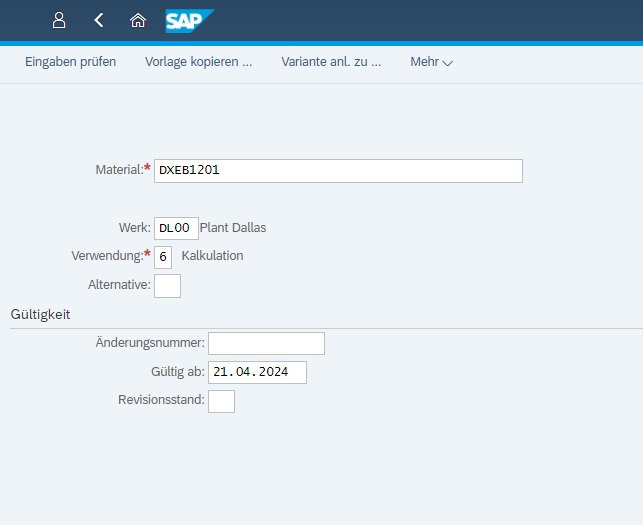
\includegraphics[width=0.9\textwidth]{Stueckliste}
    \\
    Quelle: Eigene Darstellung
\end{figure}

Nachdem \textit{Vorlage kopieren...} gewählt wurde, öffnet sich nun ein neues Fenster, in welchem man die Daten für die Vorlage eingeben muss. Im vorliegenden Beispiel sind das bei \textit{Material} der Wert 
\textit{DXTR1201} und für \textit{Verwendung} der Wert \textit{1} (Fertigung).

\begin{figure}[H]
    \caption{Vorlage kopieren}\label{fig:vorlage}
    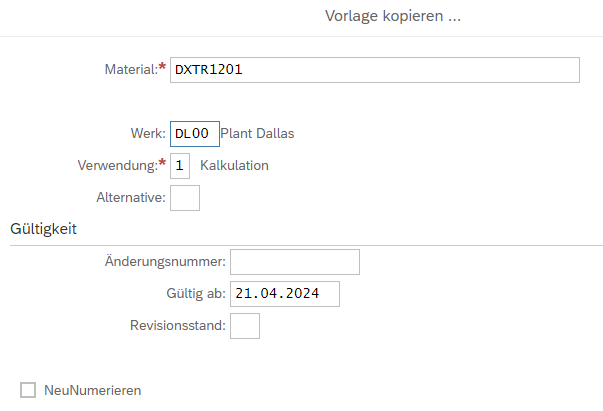
\includegraphics[width=0.9\textwidth]{Vorlage}
    \\
    Quelle: Eigene Darstellung
\end{figure}

Wenn man alle Daten korrekt angegeben hat, öffnet sich nun ein neues Fenster mit der Stückliste des Deluxe Tracking Bikes. Diese kann nun mit den neuen Materialien angepasst werden. 
Im Fallbeispiel sind dies der Elektromotor, der Akku und das Ladekabel, welche in der Spalte \textit{Komponente} mit ihren Namen \textit{EBEN1201}, \textit{EBAK1201} und \textit{EBCG1201} eingetragen werden müssen.
Weiterhin muss der Passende wert in der Spalte \textit{PTp} (Positionstyp) eingetragen werden. Im Beispiel wird hier für alle neuen Materialien der Wert \textit{N} (Nichtlagerposition) verwendet.
Man kann hier noch weitere Werte wie \textit{Menge} angeben. Da aber im Beispiel jedes der neuen Bauteile nur einmal verbaut wird, ist das hier nicht nötig. Wenn man alle Daten korrekt 
eingetragen hat, kann man auf \textit{Sichern} klicken.

\begin{figure}[H]
    \caption{Stückliste anpassen}\label{fig:stueckliste2}
    \includegraphics[width=0.9\textwidth]{Stueckliste2}
    \\
    Quelle: Eigene Darstellung
\end{figure}

\subsubsection{Anlegen des Arbeitsplans}
Nachdem die Stückliste erfolgreich angelegt wurde, kann nun ein Arbeitsplan für das E-Bike angelegt werden. Hierfür muss von der Startseite unter dem Reiter \textit{Controlling} die Kachel \textit{Arbeitsplan anlegen} gewählt werden.
Hier wird man so wie bei der Stückliste aufgefordert das Material anzugeben, für welches der Arbeitsplan erstellt werden soll. In der Fallstudie wird hier das E-Bike \textit{DXEB1201}, sowie das Werk \textit{DL00} angegeben. Außerdem 
muss man darauf achten, dass beim \textit{Stichtag} das aktuelle Datum eingetragen ist. Da das E-Bike und das Deluxe Tracking Bike im Fallbeispiel starke Ähnlichkeiten aufweisen, ist es hier empfehlenswert wieder die Vorlage des Deluxe Tracking Bikes zu verwenden.
Hierfür muss der Button \textit{Vorlage} gewählt werden.

\begin{figure}[H]
    \caption{Arbeitsplan anlegen}\label{fig:arbeitsplan}
    \includegraphics[width=0.9\textwidth]{Arbeitsplan}
    \\
    Quelle: Eigene Darstellung
\end{figure}

Anschließend öffnet sich ein neues Fenster, in welchem man, soweit nicht schon geschehen \textit{Normalarbeitsplan} auswählen muss.

\begin{figure}[H]
    \caption{Arbeitsplan anlegen - Plantyp der Vorlage}\label{fig:arbeitsplan2}
    \includegraphics[width=0.9\textwidth]{Arbeitsplan2}
    \\
    Quelle: Eigene Darstellung
\end{figure}

Daraufhin muss man das Material angeben, dessen Vorlage man verwenden will. Im Beispiel ist das \textit{DXTR1201}, und in einem weiteren Fenster hat man 
die Möglichkeit, mit dem Feld \textit{Plangruppenzähler} die Vorlage zu spezifizieren. Da es sich aber um den ersten Arbeitsplan für das E-Bike handelt, wird hier der Wert \textit{1} beibehalten.

\begin{figure}[H]
    \caption{Arbeitsplan anlegen - Vorlagenselektion}\label{fig:arbeitsplan3}
    \includegraphics[width=0.9\textwidth]{Arbeitsplan3}
    \\
    Quelle: Eigene Darstellung
\end{figure}

\begin{figure}[H]
    \caption{Arbeitsplan anlegen - Weitere Anpassungen der Vorlage}\label{fig:arbeitsplan4}
    \includegraphics[width=0.9\textwidth]{Arbeitsplan4}
    \\
    Quelle: Eigene Darstellung
\end{figure}

Wenn man jetzt fortfährt, so öffnet sich ein neues Fenster, in welchem der Arbeitsplan des Deluxe Tracking Bikes angezeigt wird. Dieser kann nun nach Bedarf angepasst werden. Im Beispiel werden hier zwischen den Arbeitsschritten 0010 und 0020, 0060 und 0070 sowie 0110 und 0120 neue Arbeitsschritte eingefügt. Diese Arbeitsschritte sind für die Montage des Elektromotors (neues 0020) und des Akkus (neues 0080) sowie dem Beilegen des Ladekabels (neues 0130). Neben der Beschreibung muss hier darauf geachtet werden, 
dass der richtige Arbeitsplan gewählt wird. Dieser ist bei Vorgang 0020 und 0080 \textit{ASSY1000} und bei Vorgang 0130 \textit{PACK1000}. Außerdem wird im Beispiel eine Schätzung für die Personalzeit abgegeben, welche sich bei Vorgang 0020 auf \textit{7} min beläuft und bei Vorgang 0080 und 0130 \textit{5} min beträgt.

\begin{figure}[H]
    \caption{Arbeitsplan anpassen}\label{fig:arbeitsplan5}
    \includegraphics[width=0.9\textwidth]{Arbeitsplan5}
    \\
    Quelle: Eigene Darstellung
\end{figure}

\subsubsection{Durchführung der Kostenkalkulation}
Nachdem die Stückliste und der Arbeitsplan erfolgreich angelegt wurden, kann nun die Kostenkalkulation durchgeführt werden. Hierfür navigiert man auf der Startseite im Reiter \textit{Controlling} zur Kachel \textit{Materialkalkulationen anlegen} und wählt diese aus.
 Im neuen Fenster müssen die Daten für die Kalkulation angegeben werden. In der Fallstudie wird im Feld \textit{Material} das E-Bike \textit{DXEB1201} und im Feld \textit{Werk} das Werk \textit{DL00} angegeben. Weiterhin wird als \textit{Kalkulationsvariante} \textit{PPC1} eingetragen. Hier wird PPC1 gewählt da es sich um ein neues Produkt handelt. Zudem wird in das Feld 
 \textit{Kalkulationsgröße} der Wert \textit{1} eingetragen.

\begin{figure}[H]
    \caption{Materialkalkulationen anlegen}\label{fig:kalkulation}
    \includegraphics[width=0.9\textwidth]{Kalkulation}
    \\
    Quelle: Eigene Darstellung
\end{figure}

In dem daraufhin geöffneten Fenster muss man nochmal sichergehen, dass das feld \textit{Kalkulationsdatum ab:} mit dem aktuellen Datum befüllt ist.

\begin{figure}[H]
    \caption{Materialkalkulationen anlegen - Kalkulationsdatum}\label{fig:kalkulation2}
    \includegraphics[width=0.9\textwidth]{Kalkulation2}
    \\
    Quelle: Eigene Darstellung
\end{figure}

Wenn man bestätigt öffnet sich jetzt ein neues Fenster, welches das Ergebnis der Kostenkalkulation anzeigt. Wichtig hierbei ist, dass es sich um reine Selbstkosten handelt. 

\begin{figure}[H]
    \caption{Materialkalkulationen anlegen - Ergebnis}\label{fig:kalkulation3}
    \includegraphics[width=0.9\textwidth]{Kalkulation3}
    \\
    Quelle: Eigene Darstellung
\end{figure}

\subsubsection{Vormerken der Preisfortschreibung}
Nachdem die Kostenkalkulation erfolgreich durchgeführt wurde, kann nun der Preis für das E-Bike vorgeschlagen werden. Hierfür muss eine Preisfortschreibung vorgemerkt werden.
 Von der Startseite aus unter dem Reiter \textit{Controlling} muss dafür die Kachel \textit{Materialkalkulationen freigeben} ausgewählt werden. Daraufhin erscheint ein Fenster in welchem man das Material, für welches die Preisfortschreibung vorgemerkt werden soll, angeben muss.
  Im Fallbeispiel wird hier als Buchungskreis \textit{US00}, als Werk \textit{DL00} und als Material \textit{DXEB1201} eingetragen und man muss darauf achten, dass im Feld \textit{Buchungsperiode/Geschäftsjahr} der aktuelle Monat angegeben ist. Außerdem ist es wichtig, dass man den Haken bei \textit{Testlauf} entfernt.

\begin{figure}[H]
    \caption{Materialkalkulationen freigeben}\label{fig:freigabe}
    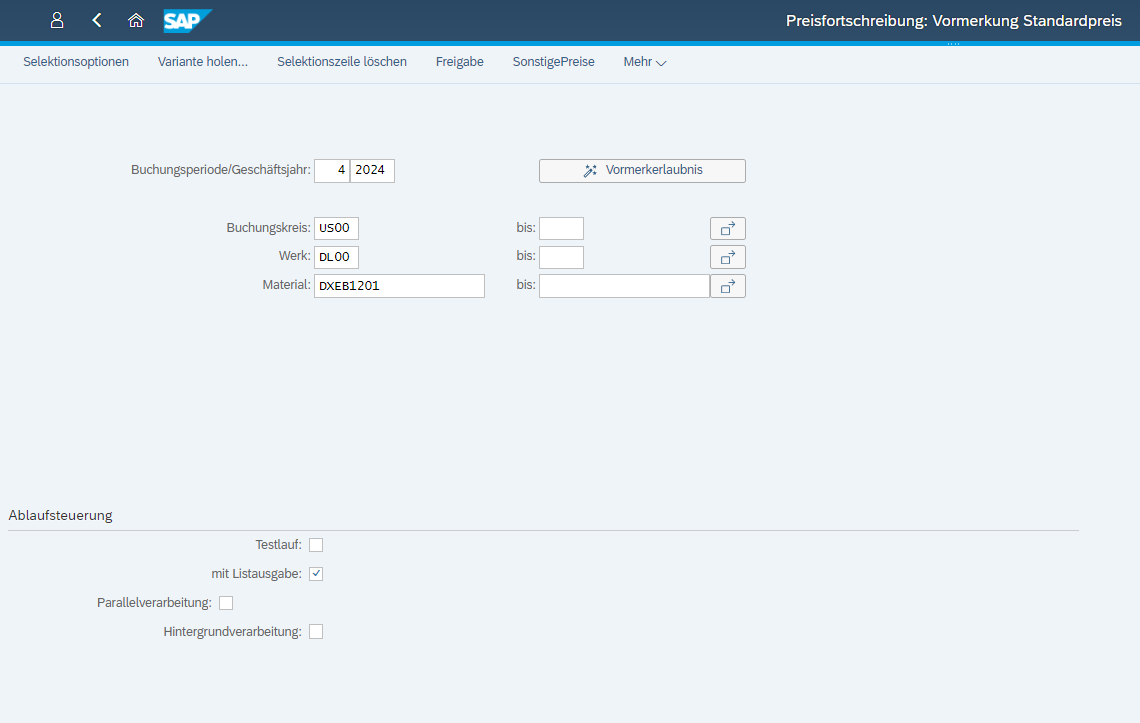
\includegraphics[width=0.9\textwidth]{Freigabe}
    \\
    Quelle: Eigene Darstellung
\end{figure}

Fährt man fort, so öffnet sich ein neues Fenster. Sollte die Preisfortschreibung erfolgreich vorgemerkt worden sein, so bekommt man in diesem Fenster eine Bestätigung. Andersfalls wird eine Fehlermeldung angezeigt.

\begin{figure}[H]
    \caption{Materialkalkulationen freigeben - Ergebnis}\label{fig:freigabe2}
    \includegraphics[width=0.9\textwidth]{Freigabe2}
    \\
    Quelle: Eigene Darstellung
\end{figure}

\subsubsection{Auswertung der Ergebnisse}
Um die Ergebnisse der Kostenkalkulation zu analysieren, kann man sich mit diesem Schritt die Ergebnisse nochmal darstellen lassen. Hierfür muss man von der Startseite aus unter 
dem Reiter \textit{Controlling} die Karte \textit{Material anzeigen} auswählen. Daraufhin wird man aufgefordert das Material anzugeben. Im Beispiel wird hier das E-Bike \textit{DXEB1201} angegeben.

\begin{figure}[H]
    \caption{Material anzeigen}\label{fig:anzeige}
    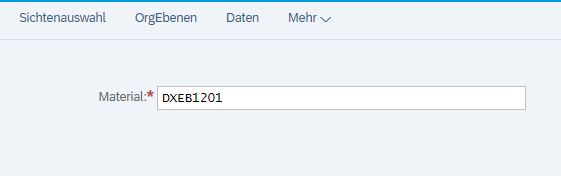
\includegraphics[width=0.9\textwidth]{Anzeige}
    \\
    Quelle: Eigene Darstellung
\end{figure}

Nachdem eingeben des Materials öffnet sich ein neues Fenster, in welchem man die Sichten wählen muss. Hier empfehlen sich die Sichten \textit{Kalkulation 1} und \textit{Kalkulation 2}. Darauf wird man aufgefordert das Werk anzugeben. Im Beispiel ist dies \textit{DL00}.
Wenn man nun den Reiter \textit{Kalkulation 2} auswählt, so sieht man in der Zeile \textit{Kalkulation} den Planpreis für das E-Bike unter \textit{Zukünftig}, sowie den Standardpreis unter \textit{Laufend} welcher beim Anlegen des Materials DXEB1201 angegeben wurde.

\begin{figure}[H]
    \caption{Material anzeigen - Kalkulation 2}\label{fig:anzeige2}
    \includegraphics[width=0.9\textwidth]{Anzeige2}
    \\
    Quelle: Eigene Darstellung
\end{figure}

\subsubsection{Freigabe der Preisfortschreibung}
Nachdem die Ergebnisse der Kostenkalkulation analysiert wurden und ein positiver Entschluss gefasst wurde, kann nun die Preisfortschreibung freigegeben werden. Hierfür Navigieren wir von der Startseite aus unter dem Reiter \textit{Controlling} zur Kachel \textit{Materialkalkulationen freigeben} und wählen diese aus.
 Im neuen Fenster werden die Felder jetzt so wie im Schritt, in dem die Preisfortschreibung vorgemerkt wurde, ausgefüllt. Anders als beim Vormerken muss nun aber auf den Button \textit{Freigabe} geklickt werden. Hier bekommt man nun wieder die Rückmeldung, ob die Freigabe erfolgreich war oder nicht. Falls die Freigabe erfolgreich war, so ist der Preis für das E-Bike nun festgelegt.
 An dieser Stelle ist die Fallstudie abgeschlossen.

\begin{figure}[H]
    \caption{Materialkalkulationen freigeben}\label{fig:freigabe3}
    \includegraphics[width=0.9\textwidth]{Freigabe3}
    \\
    Quelle: Eigene Darstellung
\end{figure}